\documentclass[conference]{IEEEtran}
\IEEEoverridecommandlockouts
% The preceding line is only needed to identify funding in the first footnote. If that is unneeded, please comment it out.
\usepackage{cite}
\usepackage{amsmath,amssymb,amsfonts}
\usepackage{algorithmic}
\usepackage{graphicx}
\usepackage{textcomp}
\usepackage{xcolor}
\def\BibTeX{{\rm B\kern-.05em{\sc i\kern-.025em b}\kern-.08em
    T\kern-.1667em\lower.7ex\hbox{E}\kern-.125emX}}
\begin{document}

\title{Implementing the Perceptron algorithm for finding the
weights of a Linear Discriminant function\\
}

\author{\IEEEauthorblockN{Devopriya Tirtho}
\IEEEauthorblockN{16.02.04.033}
\IEEEauthorblockA{\textit{Department of Computer Science and Engineering} \\
\textit{Ahsanullah University of Science and Technology}\\
Dhaka, Bangladesh \\
}

}

\maketitle

\begin{abstract}
In \textbf{'Machine Learning'}, for predicting the accurate class of an unknown sample we need to visualize our training samples whether they are linearly separable or not. \textbf{'Perceptron Algorithm'} helps to find the actual weights of a \textbf{'Linear Discriminant'} function for convergence.
\end{abstract}

\begin{IEEEkeywords}
Machine Learning, Perceptron Algorithm, Linear Discriminant, Function.
\end{IEEEkeywords}

\section{Introduction}
\textbf{‘Perceptron Algorithm’} is the type of learning algorithm which helps to find the weights to converge a linear discriminant function. In \textbf{‘Perceptron Learning Algorithm’}, the weights are updated systematically to ommit the misclassified classification. This process leads to converge the linear discriminant function so that, no point is misclassified. This algorithm works on misclassified datapoints by updating weights with a particular learning rate to converge. The learning rate may vary. 


\section{Task}

There is a dataset named 'train-perceptroptron' where all the datapoints are given. The datapoints are classified between \textbf{'two'} classes namely $'1'$ and $'2'$. Here are the datapoints of ‘train-perceptron’ dataset classified into $Class-1$ as $W1$ and $Class-2$ as $W2$:\\
	$W1$= $\{(1,1), (1, -1), (4, 5)\}$\\
	$W2$= $\{(2, 2.5), (0, 2), (2, 3)\}$\\
\begin{itemize}  
\item Firstly, we have to plot all the data points of each class with corresponding marker in graph.\\
\item Secondly, we have to apply the following $phi$ function in order to get the high dimensional sample points $y$. The $phi$ function is:\\
\begin{equation}
y= [x_1^2\textrm{   }   x_2^2\textrm{   }   x_1*x_2 \textrm{   }   x_1\textrm{   }    x_2\textrm{   }    1]
\end{equation}
\item Thirdly, we have to normalize $class\textrm{   } 2$ and then, we have to use perceptron algorithm on the dataset to find all the coefficients' weights of the discriminant function for the linear classifier. We have to find the weights in two methods. Such as: $One\textrm{   } at\textrm{   } a \textrm{   }Time$ and $Many \textrm{   }at \textrm{   }a\textrm{   } Time$ and have to vary the value of learning rate $alpha$ among $0$ to $1$ with step size $0.1$. The perceptron algorithm which we follow:\\

\begin{equation}
\tilde{W}(i+1)= \tilde{W}(i)+\alpha\tilde{Y}_m^k\\
\end{equation}
$\textrm{if}\textrm{   }\tilde{W}(i)*\alpha\tilde{Y}_m^k<=0; Misclassified$
\begin{equation}
\tilde{W}(i+1)= \tilde{W}(i)\\
\end{equation}
$\textrm{if}\textrm{   }\tilde{W}(i)*\alpha\tilde{Y}_m^k>0; Classified$

\item Finally, we have to design the perceptron algorithm for initial weights of all zero, all one and randomly initialized with seed fixed and plot all the data points in a bar chart to visualize our experiment.
\end{itemize}

\section{Experimental Design}
\begin{itemize}  
	\item \textbf{Plotting All Training Points:}
	In our given dataset which is named as ‘train’, we need to pick the values which represent X-coordinate values and Y-coordinate values. Then with appropriate marker and distinct color we have to plot the points of \textbf{‘Class 1’} and \textbf{‘Class 2’}.\\
\begin{figure}[htbp]
\centerline{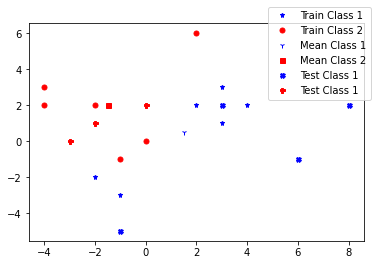
\includegraphics[scale=0.5]{11.png}}
\caption{Datapoints of Class 1 and Class 2}
\label{fig}
\end{figure}
	\item \textbf{Running Perceptron Algorithm:}
Then we have to run the perceptron algorithm for all initial weights of zero, one and randomly initialized with fixed seed respectively.\\
\item \textbf{Plotting Bar Chart for Visualization:}
After getting our desired table, we plot the data into a bar char for visualization.
\begin{table}[htbp]
\caption{Table for Initial Weight Vector of All One}
\begin{center}
\begin{tabular}{|c|c|c|}
\hline
\textbf{\textit{Alpha (Learning Rate)}}& \textbf{\textit{One at a Time}}& \textbf{\textit{Many at a Time}} \\
\hline
\textbf{{0.1}}& \textbf{{6}}& \textbf{{102}} \\
\hline
\textbf{{0.2}}& \textbf{{92}}& \textbf{{104}} \\
\hline
\textbf{{0.3}}& \textbf{{104}}& \textbf{{91}} \\
\hline
\textbf{{0.4}}& \textbf{{106}}& \textbf{{116}} \\
\hline
\textbf{{0.5}}& \textbf{{93}}& \textbf{{105}} \\
\hline
\textbf{{0.6}}& \textbf{{93}}& \textbf{{114}} \\
\hline
\textbf{{0.7}}& \textbf{{108}}& \textbf{{91}} \\
\hline
\textbf{{0.8}}& \textbf{{115}}& \textbf{{91}} \\
\hline
\textbf{{0.9}}& \textbf{{94}}& \textbf{{105}} \\
\hline
\textbf{{1.0}}& \textbf{{94}}& \textbf{{93}} \\
\hline
\end{tabular}
\label{tab1}
\end{center}
\end{table}


\begin{table}[htbp]
\caption{Table for Initial Weight Vector of All Zero}
\begin{center}
\begin{tabular}{|c|c|c|}
\hline
\textbf{\textit{Alpha (Learning Rate)}}& \textbf{\textit{One at a Time}}& \textbf{\textit{Many at a Time}} \\
\hline
\textbf{{0.1}}& \textbf{{94}}& \textbf{{105}} \\
\hline
\textbf{{0.2}}& \textbf{{94}}& \textbf{{105}} \\
\hline
\textbf{{0.3}}& \textbf{{94}}& \textbf{{92}} \\
\hline
\textbf{{0.4}}& \textbf{{94}}& \textbf{{105}} \\
\hline
\textbf{{0.5}}& \textbf{{94}}& \textbf{{92}} \\
\hline
\textbf{{0.6}}& \textbf{{94}}& \textbf{{92}} \\
\hline
\textbf{{0.7}}& \textbf{{94}}& \textbf{{92}} \\
\hline
\textbf{{0.8}}& \textbf{{94}}& \textbf{{105}} \\
\hline
\textbf{{0.9}}& \textbf{{94}}& \textbf{{105}} \\
\hline
\textbf{{1.0}}& \textbf{{94}}& \textbf{{92}} \\
\hline
\end{tabular}
\label{tab1}
\end{center}
\end{table}


\begin{table}[htbp]
\caption{Table for Initial Weight Vector of All Randomly Initialized with Fixed Seed 3}
\begin{center}
\begin{tabular}{|c|c|c|}
\hline
\textbf{\textit{Alpha (Learning Rate)}}& \textbf{\textit{One at a Time}}& \textbf{\textit{Many at a Time}} \\
\hline
\textbf{{0.1}}& \textbf{{33}}& \textbf{{48}} \\
\hline
\textbf{{0.2}}& \textbf{{21}}& \textbf{{93}} \\
\hline
\textbf{{0.3}}& \textbf{{89}}& \textbf{{107}} \\
\hline
\textbf{{0.4}}& \textbf{{10}}& \textbf{{13}} \\
\hline
\textbf{{0.5}}& \textbf{{80}}& \textbf{{10}} \\
\hline
\textbf{{0.6}}& \textbf{{8}}& \textbf{{81}} \\
\hline
\textbf{{0.7}}& \textbf{{100}}& \textbf{{89}} \\
\hline
\textbf{{0.8}}& \textbf{{93}}& \textbf{{132}} \\
\hline
\textbf{{0.9}}& \textbf{{97}}& \textbf{{7}} \\
\hline
\textbf{{1.0}}& \textbf{{98}}& \textbf{{99}} \\
\hline
\end{tabular}
\label{tab1}
\end{center}
\end{table}



\begin{figure}[htbp]
\centerline{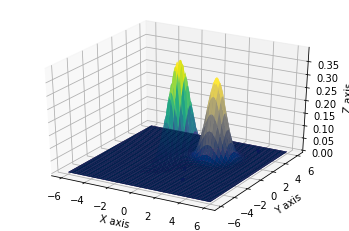
\includegraphics[scale=0.5]{12.png}}
\caption{Bar Chart with Initial Weight Vector of all One}
\label{fig}
\end{figure}

\begin{figure}[htbp]
\centerline{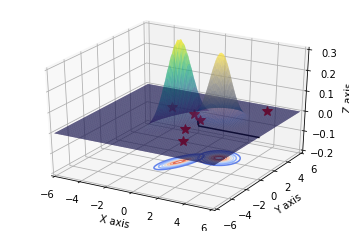
\includegraphics[scale=0.5]{13.png}}
\caption{Bar Chart with Initial Weight Vector of all Zero}
\label{fig}
\end{figure}

\begin{figure}[htbp]
\centerline{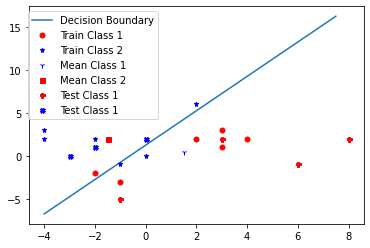
\includegraphics[scale=0.5]{14.png}}
\caption{Bar Chart with Initial Weight Vector of all Randomly Initialized Value with Seed 3}
\label{fig}
\end{figure}
\end{itemize}

\section{Answer of the Questions}
\textbf{Answers:}\\
\textbf{a.} We need to take the sample points to a high dimension to make the points separable. If we do not take the sample points to a higher dimension, they cannot be separated by a single linear line. That is why we need to take them to a high dimension.\\
\textbf{b.} In each of the three initial weight cases and for each learning rate, the number of updates is required is shown in the above table which is needed by the algorithm take before converging\\




\section{Result Analysis}
From the implemetation of the \textbf{Perceptron Algorithm} it is quite visible that when we vary the learning rate the convergence rate of $single \textrm{   }update$ and $batch\textrm{   } update$ varies. When all the initial weights are $One$ with the increment of learning rate $batch\textrm{   } update$ needs fewer iterations for convergence. $batch\textrm{   } update$ converges faster than
$single \textrm{   }update$ $four$ times when all the weight vectors are initialized with $one$. When the weight vector is initialized with $zero$, for all learning rate  $single \textrm{   }update$ needs $ninety-four$ iterations to converge and $batch\textrm{   } update$ needs higher number of interations for convergence. For random initialization, $single \textrm{   }update$ converges $seven$ times faster than $batch\textrm{   } update.$


\section{Python Code}
\begin{figure}[htbp]
\centerline{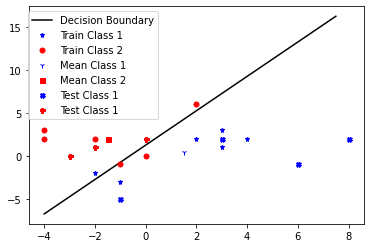
\includegraphics[scale=0.5]{16.png}}
\centerline{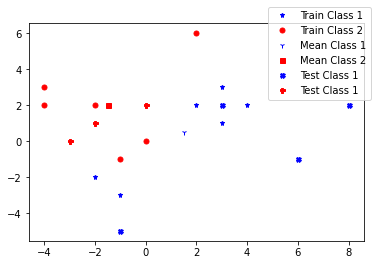
\includegraphics[scale=0.5]{17.png}}
\centerline{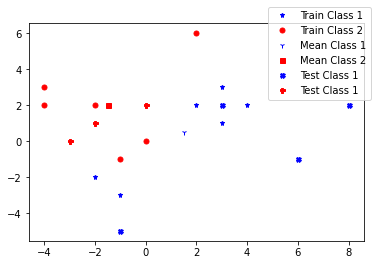
\includegraphics[scale=0.5]{19.png}}

\caption{Snapshot of python code}
\label{fig}
\end{figure}


\section{Conclusion}

\textbf{‘Perceptron Algorithm’} is a simple classification technique which uses linear discriminant function to update the misclassified weights to converge the function accurately. This algorithm works on the misclassified datapoints and helps to find the actual weight vector for the classification model.




\end{document}
